\usetikzlibrary{positioning}


\begin{frame}{Rendering Architecture}
    \centering
    % Define the style for the boxes
    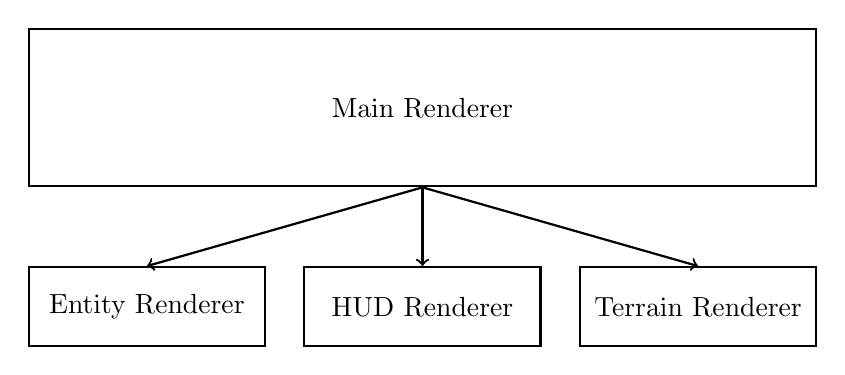
\begin{tikzpicture}
        % Main Renderer
        \node[draw, thick, minimum width=10cm, minimum height=2cm] (main) {Main Renderer};

        % Subrenderers: TerrainRenderer, HUDRenderer, EntityRenderer
        \node[draw, thick, minimum width=3cm, minimum height=1cm, below=1cm of main, xshift=-3.5cm] (entity) {Entity Renderer};
        \node[draw, thick, minimum width=3cm, minimum height=1cm, below=1cm of main] (hud) {HUD Renderer};
        \node[draw, thick, minimum width=3cm, minimum height=1cm, below=1cm of main, xshift=3.5cm] (terrain) {Terrain Renderer};

        % Arrows from main renderer to subrenderers
        \draw[->, thick] (main.south) -- (entity.north);
        \draw[->, thick] (main.south) -- (terrain.north);
        \draw[->, thick] (main.south) -- (hud.north);
    \end{tikzpicture}
\end{frame}

\begin{frame}{Rendering Architecture - Normal Mode}
    \includegraphics[width=\textwidth]{../figures/Ingame-Picture.png}
\end{frame}

\begin{frame}{Rendering Architecture - Entity Renderer}
    \begin{itemize}
        \item Entities are rendered with their respective textures
        \item Handles animations of the Entites, e.g. walking
    \end{itemize}
    \vspace{1cm}
    \centering
    \includegraphics[width=0.7\textwidth]{../../assets/texture/player_walk.png}
\end{frame}

\begin{frame}{Rendering Architecture - Terrain Renderer}
    \begin{itemize}
        \item Terrain is continuously rendered with a texture
    \end{itemize}
    \vspace{1cm}
    \centering
    \includegraphics[width=0.4\textwidth]{../../assets/layers/mountain3.png}
\end{frame}

\begin{frame}{Rendering Architecture - HUD Renderer}
    \begin{itemize}
        \item Heads-Up-Display (HUD) is rendered on top of the game
        \item Displays the player's health, score, inventory etc.
    \end{itemize}

    \vspace{1cm}
    \centering
    \begin{tabular}{ccc}
        \rotatebox{0}{\includegraphics[width=0.2\textwidth]{../../assets/texture/coin.png}} &
        \includegraphics[width=0.2\textwidth]{../../assets/texture/kaiserschmarrn.png} &
        \rotatebox{0}{\includegraphics[width=0.2\textwidth]{../../assets/texture/duck.png}}
    \end{tabular}
\end{frame}


\begin{frame}{Rendering Architecture - Debug Mode}
    \includegraphics[width=\textwidth]{../figures/Debug-Mode.png}
\end{frame}